\documentclass{standalone}
\usepackage{tikz}
\usetikzlibrary{patterns, positioning}
\usepackage[sfdefault]{ClearSans} %% option 'sfdefault' activates Clear Sans as the default text font
\usepackage[T1]{fontenc}

\begin{document}
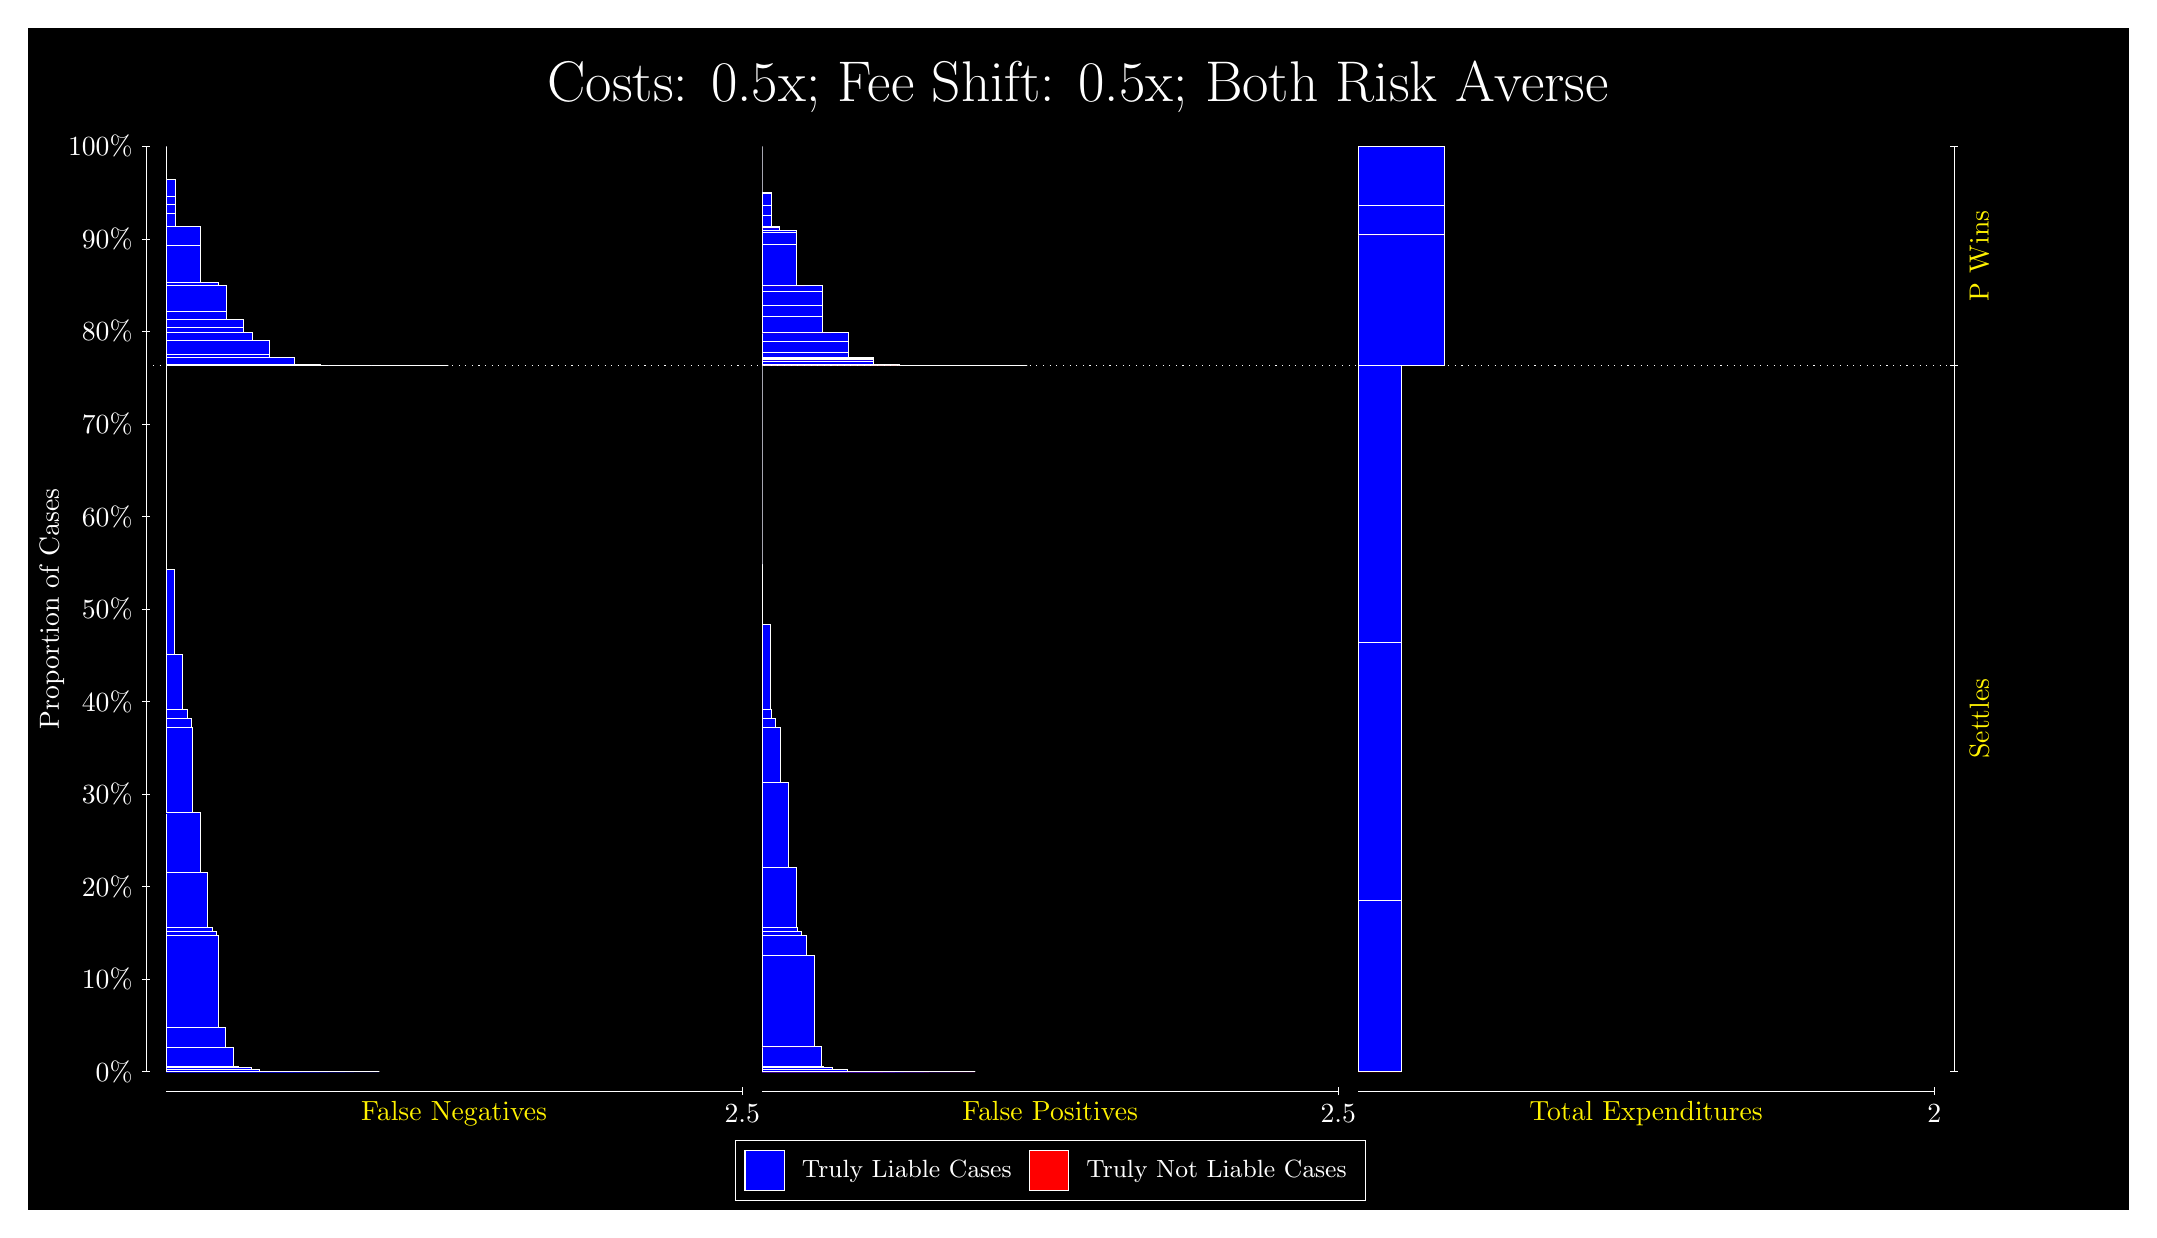
\begin{tikzpicture}
\draw[fill=black] (0,0) rectangle (26.667,15);
\draw[text=white] (0,13.5) rectangle (26.667,15) node[midway] {\huge Costs: 0.5x; Fee Shift: 0.5x; Both Risk Averse};
\draw[white, very thin] (1.5,1.75) -- (1.5,13.5);
\node[rotate=90, text=white, anchor=center] at (0.3, 7.625) {Proportion of Cases};
\draw[white, very thin] (1.45,1.75) -- (1.55,1.75);
\node[text=white, anchor=east] at (1.45, 1.75) {0\%};
\draw[white, very thin] (1.45,2.925) -- (1.55,2.925);
\node[text=white, anchor=east] at (1.45, 2.925) {10\%};
\draw[white, very thin] (1.45,4.1) -- (1.55,4.1);
\node[text=white, anchor=east] at (1.45, 4.1) {20\%};
\draw[white, very thin] (1.45,5.275) -- (1.55,5.275);
\node[text=white, anchor=east] at (1.45, 5.275) {30\%};
\draw[white, very thin] (1.45,6.45) -- (1.55,6.45);
\node[text=white, anchor=east] at (1.45, 6.45) {40\%};
\draw[white, very thin] (1.45,7.625) -- (1.55,7.625);
\node[text=white, anchor=east] at (1.45, 7.625) {50\%};
\draw[white, very thin] (1.45,8.8) -- (1.55,8.8);
\node[text=white, anchor=east] at (1.45, 8.8) {60\%};
\draw[white, very thin] (1.45,9.975) -- (1.55,9.975);
\node[text=white, anchor=east] at (1.45, 9.975) {70\%};
\draw[white, very thin] (1.45,11.15) -- (1.55,11.15);
\node[text=white, anchor=east] at (1.45, 11.15) {80\%};
\draw[white, very thin] (1.45,12.325) -- (1.55,12.325);
\node[text=white, anchor=east] at (1.45, 12.325) {90\%};
\draw[white, very thin] (1.45,13.5) -- (1.55,13.5);
\node[text=white, anchor=east] at (1.45, 13.5) {100\%};

\draw[white, very thin] (24.457,1.75) -- (24.457,13.5);
\draw[white, very thin] (24.407,1.75) -- (24.507,1.75);
\node[anchor=west] at (24.407, 1.75) {};
\draw[white, very thin] (24.407,10.719) -- (24.507,10.719);
\node[anchor=west] at (24.407, 10.719) {};
\draw[white, very thin] (24.407,13.5) -- (24.507,13.5);
\node[anchor=west] at (24.407, 13.5) {};

\draw[white, very thin, fill=blue] (1.75,1.75) rectangle (4.458,1.75);
\draw[white, very thin, fill=blue] (1.75,1.75) rectangle (4.1327,1.75);
\draw[white, very thin, fill=blue] (1.75,1.75) rectangle (4.0188,1.75);
\draw[white, very thin, fill=blue] (1.75,1.75) rectangle (3.8074,1.75);
\draw[white, very thin, fill=blue] (1.75,1.75) rectangle (3.6936,1.75);
\draw[white, very thin, fill=blue] (1.75,1.75) rectangle (3.5797,1.75);
\draw[white, very thin, fill=blue] (1.75,1.75) rectangle (3.4821,1.75);
\draw[white, very thin, fill=blue] (1.75,1.75) rectangle (3.4333,1.75);
\draw[white, very thin, fill=blue] (1.75,1.75) rectangle (3.3683,1.75);
\draw[white, very thin, fill=blue] (1.75,1.75) rectangle (3.2544,1.7506);
\draw[white, very thin, fill=blue] (1.75,1.7506) rectangle (3.1568,1.7511);
\draw[white, very thin, fill=blue] (1.75,1.7511) rectangle (3.1081,1.7511);
\draw[white, very thin, fill=blue] (1.75,1.7511) rectangle (3.043,1.7512);
\draw[white, very thin, fill=blue] (1.75,1.7512) rectangle (2.9942,1.7516);
\draw[white, very thin, fill=blue] (1.75,1.7516) rectangle (2.9292,1.7761);
\draw[white, very thin, fill=blue] (1.75,1.7761) rectangle (2.8316,1.8004);
\draw[white, very thin, fill=blue] (1.75,1.8004) rectangle (2.7828,1.8004);
\draw[white, very thin, fill=blue] (1.75,1.8004) rectangle (2.7177,1.8067);
\draw[white, very thin, fill=blue] (1.75,1.8067) rectangle (2.6689,1.8139);
\draw[white, very thin, fill=blue] (1.75,1.8139) rectangle (2.6039,2.0623);
\draw[white, very thin, fill=blue] (1.75,2.0623) rectangle (2.5063,2.3128);
\draw[white, very thin, fill=blue] (1.75,2.3128) rectangle (2.4575,2.3129);
\draw[white, very thin, fill=blue] (1.75,2.3129) rectangle (2.4087,3.477);
\draw[white, very thin, fill=blue] (1.75,3.477) rectangle (2.3924,3.5308);
\draw[white, very thin, fill=blue] (1.75,3.5308) rectangle (2.3436,3.5852);
\draw[white, very thin, fill=blue] (1.75,3.5852) rectangle (2.2786,4.2828);
\draw[white, very thin, fill=blue] (1.75,4.2828) rectangle (2.181,5.0385);
\draw[white, very thin, fill=blue] (1.75,5.0385) rectangle (2.1322,5.039);
\draw[white, very thin, fill=blue] (1.75,5.039) rectangle (2.0834,6.1227);
\draw[white, very thin, fill=blue] (1.75,6.1227) rectangle (2.0672,6.2344);
\draw[white, very thin, fill=blue] (1.75,6.2344) rectangle (2.0184,6.3461);
\draw[white, very thin, fill=blue] (1.75,6.3461) rectangle (1.9533,7.0437);
\draw[white, very thin, fill=blue] (1.75,7.0437) rectangle (1.8557,8.1274);
\draw[white, very thin, fill=blue] (1.75,8.1274) rectangle (1.8069,8.1278);
\draw[white, very thin, fill=blue] (1.75,8.1278) rectangle (1.7581,8.8836);
\draw[white, very thin, fill=red] (1.75,8.8836) rectangle (1.75,8.8836);
\draw[white, very thin, fill=blue] (1.75,8.8836) rectangle (1.75,10.719);
\draw[white, very thin, fill=blue] (1.75,10.719) rectangle (5.3362,10.719);
\draw[white, very thin, fill=blue] (1.75,10.719) rectangle (5.011,10.719);
\draw[white, very thin, fill=blue] (1.75,10.719) rectangle (4.6857,10.719);
\draw[white, very thin, fill=blue] (1.75,10.719) rectangle (4.4661,10.719);
\draw[white, very thin, fill=blue] (1.75,10.719) rectangle (4.3604,10.719);
\draw[white, very thin, fill=blue] (1.75,10.719) rectangle (4.1408,10.719);
\draw[white, very thin, fill=blue] (1.75,10.719) rectangle (4.0351,10.72);
\draw[white, very thin, fill=blue] (1.75,10.72) rectangle (4.0351,10.721);
\draw[white, very thin, fill=blue] (1.75,10.721) rectangle (3.8155,10.721);
\draw[white, very thin, fill=blue] (1.75,10.721) rectangle (3.8155,10.721);
\draw[white, very thin, fill=blue] (1.75,10.721) rectangle (3.7098,10.727);
\draw[white, very thin, fill=blue] (1.75,10.727) rectangle (3.7098,10.736);
\draw[white, very thin, fill=blue] (1.75,10.736) rectangle (3.4903,10.736);
\draw[white, very thin, fill=blue] (1.75,10.736) rectangle (3.3845,10.82);
\draw[white, very thin, fill=blue] (1.75,10.82) rectangle (3.165,10.823);
\draw[white, very thin, fill=blue] (1.75,10.823) rectangle (3.165,10.827);
\draw[white, very thin, fill=blue] (1.75,10.827) rectangle (3.0593,10.862);
\draw[white, very thin, fill=blue] (1.75,10.862) rectangle (3.0593,11.033);
\draw[white, very thin, fill=blue] (1.75,11.033) rectangle (2.8397,11.133);
\draw[white, very thin, fill=blue] (1.75,11.133) rectangle (2.734,11.199);
\draw[white, very thin, fill=blue] (1.75,11.199) rectangle (2.734,11.307);
\draw[white, very thin, fill=blue] (1.75,11.307) rectangle (2.5144,11.402);
\draw[white, very thin, fill=blue] (1.75,11.402) rectangle (2.5144,11.734);
\draw[white, very thin, fill=blue] (1.75,11.734) rectangle (2.4087,11.779);
\draw[white, very thin, fill=blue] (1.75,11.779) rectangle (2.1891,12.243);
\draw[white, very thin, fill=blue] (1.75,12.243) rectangle (2.1891,12.484);
\draw[white, very thin, fill=blue] (1.75,12.484) rectangle (2.0834,12.488);
\draw[white, very thin, fill=blue] (1.75,12.488) rectangle (1.8638,12.646);
\draw[white, very thin, fill=blue] (1.75,12.646) rectangle (1.8638,12.766);
\draw[white, very thin, fill=blue] (1.75,12.766) rectangle (1.8638,12.862);
\draw[white, very thin, fill=blue] (1.75,12.862) rectangle (1.8638,13.086);
\draw[white, very thin, fill=blue] (1.75,13.086) rectangle (1.7581,13.086);
\draw[white, very thin, fill=red] (1.75,13.086) rectangle (1.75,13.086);
\draw[white, very thin, fill=blue] (1.75,13.086) rectangle (1.75,13.5);
\draw[white, very thin, fill=red] (9.3189,1.75) rectangle (12.027,1.75);
\draw[white, very thin, fill=blue] (9.3189,1.75) rectangle (12.027,1.75);
\draw[white, very thin, fill=blue] (9.3189,1.75) rectangle (11.702,1.75);
\draw[white, very thin, fill=red] (9.3189,1.75) rectangle (11.441,1.75);
\draw[white, very thin, fill=blue] (9.3189,1.75) rectangle (11.441,1.75);
\draw[white, very thin, fill=blue] (9.3189,1.75) rectangle (11.376,1.75);
\draw[white, very thin, fill=blue] (9.3189,1.75) rectangle (11.116,1.75);
\draw[white, very thin, fill=blue] (9.3189,1.75) rectangle (11.051,1.75);
\draw[white, very thin, fill=red] (9.3189,1.75) rectangle (11.002,1.75);
\draw[white, very thin, fill=blue] (9.3189,1.75) rectangle (11.002,1.75);
\draw[white, very thin, fill=red] (9.3189,1.75) rectangle (10.856,1.75);
\draw[white, very thin, fill=blue] (9.3189,1.75) rectangle (10.856,1.75);
\draw[white, very thin, fill=blue] (9.3189,1.75) rectangle (10.791,1.75);
\draw[white, very thin, fill=blue] (9.3189,1.75) rectangle (10.726,1.7505);
\draw[white, very thin, fill=blue] (9.3189,1.7505) rectangle (10.677,1.7505);
\draw[white, very thin, fill=blue] (9.3189,1.7505) rectangle (10.531,1.7511);
\draw[white, very thin, fill=blue] (9.3189,1.7511) rectangle (10.465,1.7512);
\draw[white, very thin, fill=red] (9.3189,1.7512) rectangle (10.417,1.7512);
\draw[white, very thin, fill=blue] (9.3189,1.7512) rectangle (10.417,1.7516);
\draw[white, very thin, fill=blue] (9.3189,1.7516) rectangle (10.4,1.7759);
\draw[white, very thin, fill=blue] (9.3189,1.7759) rectangle (10.352,1.7759);
\draw[white, very thin, fill=blue] (9.3189,1.7759) rectangle (10.205,1.8004);
\draw[white, very thin, fill=blue] (9.3189,1.8004) rectangle (10.14,1.8067);
\draw[white, very thin, fill=blue] (9.3189,1.8067) rectangle (10.091,1.8139);
\draw[white, very thin, fill=blue] (9.3189,1.8139) rectangle (10.075,2.0645);
\draw[white, very thin, fill=blue] (9.3189,2.0645) rectangle (10.026,2.0645);
\draw[white, very thin, fill=red] (9.3189,2.0645) rectangle (9.9776,2.0645);
\draw[white, very thin, fill=blue] (9.3189,2.0645) rectangle (9.9776,3.2286);
\draw[white, very thin, fill=blue] (9.3189,3.2286) rectangle (9.88,3.477);
\draw[white, very thin, fill=blue] (9.3189,3.477) rectangle (9.8149,3.5307);
\draw[white, very thin, fill=blue] (9.3189,3.5307) rectangle (9.7661,3.5852);
\draw[white, very thin, fill=blue] (9.3189,3.5852) rectangle (9.7499,4.3409);
\draw[white, very thin, fill=blue] (9.3189,4.3409) rectangle (9.7011,4.3414);
\draw[white, very thin, fill=blue] (9.3189,4.3414) rectangle (9.6523,5.4251);
\draw[white, very thin, fill=blue] (9.3189,5.4251) rectangle (9.5547,6.1227);
\draw[white, very thin, fill=blue] (9.3189,6.1227) rectangle (9.4896,6.2344);
\draw[white, very thin, fill=blue] (9.3189,6.2344) rectangle (9.4408,6.3461);
\draw[white, very thin, fill=blue] (9.3189,6.3461) rectangle (9.4246,7.4298);
\draw[white, very thin, fill=blue] (9.3189,7.4298) rectangle (9.3758,7.4303);
\draw[white, very thin, fill=blue] (9.3189,7.4303) rectangle (9.327,8.186);
\draw[white, very thin, fill=blue] (9.3189,8.186) rectangle (9.3189,10.719);
\draw[white, very thin, fill=red] (9.3189,10.719) rectangle (12.686,10.719);
\draw[white, very thin, fill=blue] (9.3189,10.719) rectangle (12.686,10.719);
\draw[white, very thin, fill=red] (9.3189,10.719) rectangle (12.36,10.719);
\draw[white, very thin, fill=blue] (9.3189,10.719) rectangle (12.36,10.719);
\draw[white, very thin, fill=red] (9.3189,10.719) rectangle (12.035,10.719);
\draw[white, very thin, fill=blue] (9.3189,10.719) rectangle (12.035,10.719);
\draw[white, very thin, fill=blue] (9.3189,10.719) rectangle (12.035,10.719);
\draw[white, very thin, fill=blue] (9.3189,10.719) rectangle (12.035,10.719);
\draw[white, very thin, fill=red] (9.3189,10.719) rectangle (11.71,10.719);
\draw[white, very thin, fill=blue] (9.3189,10.719) rectangle (11.71,10.719);
\draw[white, very thin, fill=blue] (9.3189,10.719) rectangle (11.71,10.719);
\draw[white, very thin, fill=red] (9.3189,10.719) rectangle (11.384,10.719);
\draw[white, very thin, fill=blue] (9.3189,10.719) rectangle (11.384,10.719);
\draw[white, very thin, fill=blue] (9.3189,10.719) rectangle (11.384,10.721);
\draw[white, very thin, fill=blue] (9.3189,10.721) rectangle (11.059,10.726);
\draw[white, very thin, fill=red] (9.3189,10.726) rectangle (11.059,10.726);
\draw[white, very thin, fill=blue] (9.3189,10.726) rectangle (11.059,10.73);
\draw[white, very thin, fill=blue] (9.3189,10.73) rectangle (11.059,10.736);
\draw[white, very thin, fill=red] (9.3189,10.736) rectangle (10.84,10.736);
\draw[white, very thin, fill=blue] (9.3189,10.736) rectangle (10.84,10.736);
\draw[white, very thin, fill=blue] (9.3189,10.736) rectangle (10.734,10.765);
\draw[white, very thin, fill=blue] (9.3189,10.765) rectangle (10.734,10.79);
\draw[white, very thin, fill=red] (9.3189,10.79) rectangle (10.734,10.79);
\draw[white, very thin, fill=blue] (9.3189,10.79) rectangle (10.734,10.812);
\draw[white, very thin, fill=blue] (9.3189,10.812) rectangle (10.734,10.827);
\draw[white, very thin, fill=red] (9.3189,10.827) rectangle (10.514,10.827);
\draw[white, very thin, fill=blue] (9.3189,10.827) rectangle (10.514,10.827);
\draw[white, very thin, fill=blue] (9.3189,10.827) rectangle (10.514,10.827);
\draw[white, very thin, fill=blue] (9.3189,10.827) rectangle (10.409,10.89);
\draw[white, very thin, fill=red] (9.3189,10.89) rectangle (10.409,10.89);
\draw[white, very thin, fill=blue] (9.3189,10.89) rectangle (10.409,11.019);
\draw[white, very thin, fill=blue] (9.3189,11.019) rectangle (10.409,11.03);
\draw[white, very thin, fill=blue] (9.3189,11.03) rectangle (10.409,11.133);
\draw[white, very thin, fill=red] (9.3189,11.133) rectangle (10.189,11.133);
\draw[white, very thin, fill=blue] (9.3189,11.133) rectangle (10.189,11.133);
\draw[white, very thin, fill=blue] (9.3189,11.133) rectangle (10.189,11.133);
\draw[white, very thin, fill=blue] (9.3189,11.133) rectangle (10.083,11.336);
\draw[white, very thin, fill=blue] (9.3189,11.336) rectangle (10.083,11.476);
\draw[white, very thin, fill=blue] (9.3189,11.476) rectangle (10.083,11.655);
\draw[white, very thin, fill=blue] (9.3189,11.655) rectangle (10.083,11.73);
\draw[white, very thin, fill=red] (9.3189,11.73) rectangle (9.8637,11.73);
\draw[white, very thin, fill=blue] (9.3189,11.73) rectangle (9.8637,11.734);
\draw[white, very thin, fill=blue] (9.3189,11.734) rectangle (9.8637,11.734);
\draw[white, very thin, fill=blue] (9.3189,11.734) rectangle (9.758,12.261);
\draw[white, very thin, fill=blue] (9.3189,12.261) rectangle (9.758,12.409);
\draw[white, very thin, fill=blue] (9.3189,12.409) rectangle (9.758,12.439);
\draw[white, very thin, fill=blue] (9.3189,12.439) rectangle (9.5384,12.466);
\draw[white, very thin, fill=red] (9.3189,12.466) rectangle (9.5384,12.466);
\draw[white, very thin, fill=blue] (9.3189,12.466) rectangle (9.5384,12.47);
\draw[white, very thin, fill=blue] (9.3189,12.47) rectangle (9.5384,12.484);
\draw[white, very thin, fill=blue] (9.3189,12.484) rectangle (9.4327,12.625);
\draw[white, very thin, fill=blue] (9.3189,12.625) rectangle (9.4327,12.745);
\draw[white, very thin, fill=blue] (9.3189,12.745) rectangle (9.4327,12.908);
\draw[white, very thin, fill=blue] (9.3189,12.908) rectangle (9.4327,12.912);
\draw[white, very thin, fill=blue] (9.3189,12.912) rectangle (9.3189,13.5);
\draw[white, very thin, fill=red] (16.888,1.75) rectangle (17.437,1.75);
\draw[white, very thin, fill=blue] (16.888,1.75) rectangle (17.437,3.9262);
\draw[white, very thin, fill=red] (16.888,3.9262) rectangle (17.437,3.9262);
\draw[white, very thin, fill=blue] (16.888,3.9262) rectangle (17.437,7.206);
\draw[white, very thin, fill=red] (16.888,7.206) rectangle (17.437,7.206);
\draw[white, very thin, fill=blue] (16.888,7.206) rectangle (17.437,10.719);
\draw[white, very thin, fill=red] (16.888,10.719) rectangle (17.986,10.719);
\draw[white, very thin, fill=blue] (16.888,10.719) rectangle (17.986,12.377);
\draw[white, very thin, fill=red] (16.888,12.377) rectangle (17.986,12.377);
\draw[white, very thin, fill=blue] (16.888,12.377) rectangle (17.986,12.75);
\draw[white, very thin, fill=red] (16.888,12.75) rectangle (17.986,12.75);
\draw[white, very thin, fill=blue] (16.888,12.75) rectangle (17.986,13.5);
\draw[white, dotted] (1.5,10.719) -- (24.457,10.719);
\draw[white, very thin] (1.75,1.5) -- (9.0689,1.5);
\node[text=yellow, anchor=north] at (5.4094, 1.5) {False Negatives};
\draw[white, very thin] (9.0689,1.45) -- (9.0689,1.55);
\node[text=white, anchor=north] at (9.0689, 1.45) {2.5};

\draw[white, very thin] (9.3189,1.5) -- (16.638,1.5);
\node[text=yellow, anchor=north] at (12.978, 1.5) {False Positives};
\draw[white, very thin] (16.638,1.45) -- (16.638,1.55);
\node[text=white, anchor=north] at (16.638, 1.45) {2.5};

\draw[white, very thin] (16.888,1.5) -- (24.207,1.5);
\node[text=yellow, anchor=north] at (20.547, 1.5) {Total Expenditures};
\draw[white, very thin] (24.207,1.45) -- (24.207,1.55);
\node[text=white, anchor=north] at (24.207, 1.45) {2};

\node[text=yellow, centered, rotate=90] at (24.777, 6.2344) {Settles};
\node[text=yellow, centered, rotate=90] at (24.777, 12.109) {P Wins};

\draw (12.978300999999998,1.5) node[draw=none] (baseCoordinate) {};
\begin{scope}[align=center]
        \matrix[scale=0.5, draw=white, below=0.5cm of baseCoordinate, nodes={draw}, column sep=0.1cm]{
            \node[rectangle, draw, minimum width=0.5cm, minimum height=0.5cm, fill=blue] {}; &
            \node[draw=none, font=\small, text=white] (B) {Truly Liable Cases}; &
            \node[rectangle, draw, minimum width=0.5cm, minimum height=0.5cm, fill=red] {}; &
            \node[draw=none, font=\small, text=white] (B) {Truly Not Liable Cases}; \\
            };
\end{scope}

\end{tikzpicture}
\end{document}